\section{Modèles Interprétables}

\subsection{Régression Linéaire}

L'avantage principal des modèles de régression linéaire est la linéarité: cela rend la procédure d'estimation simple et, surtout, ces équations linéaires ont une interprétation facile à comprendre au niveau modulaire (c'est-à-dire les poids). C'est une des principales raisons pour lesquelles le modèle linéaire et tous les modèles similaires sont si répandus dans les domaines académiques tels que la médecine, la sociologie, la psychologie, et bien d'autres domaines de recherche quantitative.

Si le modèle est le "bon" modèle dépend de si les relations dans les données répondent à certaines hypothèses:

\begin{itemize}
    \item \textbf{Linéarité:} Le modèle de régression linéaire contraint la prédiction à être une combinaison linéaire des variables.
    \item \textbf{Normalité:} On suppose que le résultat cible, étant donné les variables, suit une distribution normale.
    \item \textbf{Homoscédasticité:} On suppose que la variance des termes d'erreur est constante sur tout l'espace des variables.
    \item \textbf{Indépendance:} On suppose que chaque instance est indépendante de toute autre instance.
    \item \textbf{variables fixes:} Les variables d'entrée sont considérées comme "fixes". Par fixe, on entend qu'elles sont traitées comme des "constantes données" et non comme des variabless statistiques. Sans cette hypothèse, vous devriez ajuster des modèles d'erreur de mesure très complexes.
    \item \textbf{Absence de multicolinéarité:} Vous ne voulez pas de variables fortement corrélées car cela perturbe l'estimation des poids.
\end{itemize}

\textbf{Interprétation:}

\begin{itemize}
    \item \textbf{Variable numérique:} Augmenter la variable numérique d'une unité change le résultat estimé de son poids.
    \item \textbf{Variable binaire:} Changer la variable de la catégorie de référence à l'autre catégorie change le résultat estimé du poids de la variable.
    \item \textbf{Interception \( \beta_0 \):} L'interception est le poids de la "variable constante", qui est toujours 1 pour toutes les instances. L'interception reflète donc le résultat prédit d'une instance où toutes les variables sont à leur valeur moyenne.
\end{itemize}

\subsubsection{R-Carré}

Le \( R^2 \) vous indique quelle partie de la variance totale de votre résultat cible est expliquée par le modèle. Plus \( R^2 \) est élevé, mieux votre modèle explique les données.

La formule pour calculer \( R^2 \) est: 

\[
R^2 = 1 - \frac{SSE}{SST}
\]

où, 

\[
SSE = \sum_{i=1}^n (y^{(i)} - \hat{y}^{(i)})^2
\]

et

\[
SST = \sum_{i=1}^n (y^{(i)} - \bar{y})^2
\]

\( SSE \) vous indique combien de variance reste après avoir ajusté le modèle linéaire. \( SST \) est la variance totale du résultat cible. \( R^2 \) varie entre 0 et 1.

Il y a un piège car \( R^2 \) augmente avec le nombre de variables dans le modèle, même si elles ne contiennent aucune information sur la valeur cible. 

Il est donc préférable d'utiliser le \( R^2 \) ajusté, qui prend en compte le nombre de variables utilisées dans le modèle. Sa formule est: 

\[
\bar{R}^2 = 1 - (1 - R^2) \frac{n-1}{n-p-1}
\]

où p est le nombre de variables et n le nombre d'instances.

Il n'est pas pertinent d'interpréter un modèle avec un \( R^2 \) (ajusté) très faible, car un tel modèle n'explique essentiellement pas la variance. Toute interprétation des poids ne serait pas significative.

\subsubsection{Importance des variables}

L'importance d'une variable dans un modèle de régression linéaire peut être mesurée par la valeur absolue de sa t-statistique. La t-statistique est le poids estimé mis à l'échelle avec son erreur standard.

\[
t_{\hat{\beta}_j} = \frac{\hat{\beta}_j}{SE(\hat{\beta}_j)}
\]

Examinons ce que cette formule nous indique:
L'importance d'une variable augmente avec l'augmentation du poids.
Cela a du sens.
Plus le poids estimé a de variance (c'est-à-dire moins nous sommes certains de la valeur correcte), moins la variable est importante.
Cela a aussi du sens.

\subsubsection{Interprétation Visuelle}

\textbf{Graphique des Poids:} L'information du tableau des poids (estimations des poids et des variances) peut être visualisée dans un graphique des poids.

\textbf{Graphique des Effets:} Les effets sont le poids par variable multiplié par la valeur de la variable d'une instance (cela nous permet de supprimer tout effet de changement d'échelle):

\[
\text{effect}_{j}^{(i)} = w_{j}x_{j}^{(i)}
\]

La boîte dans un boxplot contient la gamme d'effets pour la moitié des données (de 25\% à 75\% des quantiles d'effet).
La ligne verticale dans la boîte est l'effet médian, c'est-à-dire que 50\% des instances ont un effet inférieur et l'autre moitié un effet supérieur sur la prédiction.
Les points sont des valeurs aberrantes, définies comme des points qui sont plus de \(1.5 \times \text{IQR}\) (intervalle interquartile, c'est-à-dire la différence entre le premier et le troisième quartiles) au-dessus du troisième quartile, ou moins de \(1.5 \times \text{IQR}\) sous le premier quartile.
Les deux lignes horizontales, appelées les moustaches inférieure et supérieure, relient les points sous le premier quartile et au-dessus du troisième quartile qui ne sont pas des valeurs aberrantes.
Si il n'y a pas de valeurs aberrantes, les moustaches s'étendront jusqu'aux valeurs minimale et maximale.

\hspace{3cm}
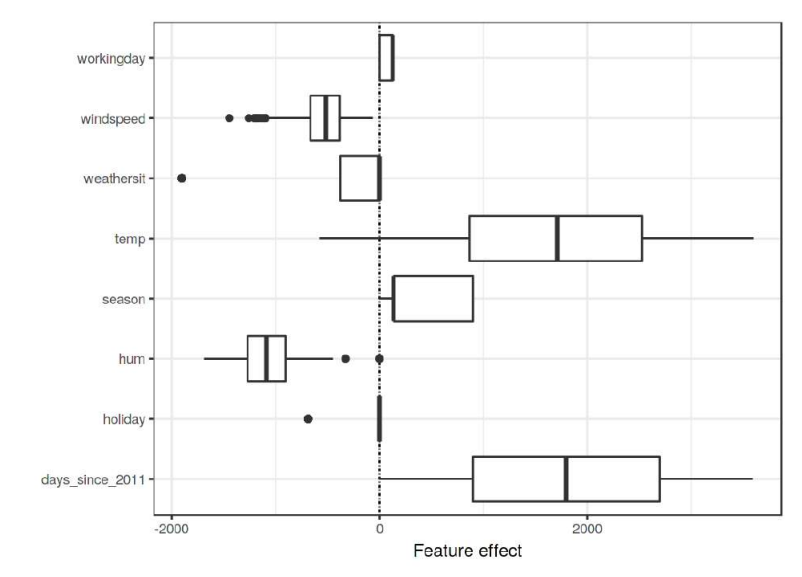
\includegraphics[width=0.5\linewidth]{Images/effect_plot.png} 
\begin{center}
    \textbf{Figure 2:} Boîtes à moustache des effets 
    \vspace{1cm}
\end{center}

\subsubsection{Expliquer les Prédictions Individuelles}

Pour obtenir les effets des variables d'une instance spécifique, nous devons multiplier ses valeurs de variables par les poids correspondants du modèle de régression linéaire.

\hspace{1.5cm}
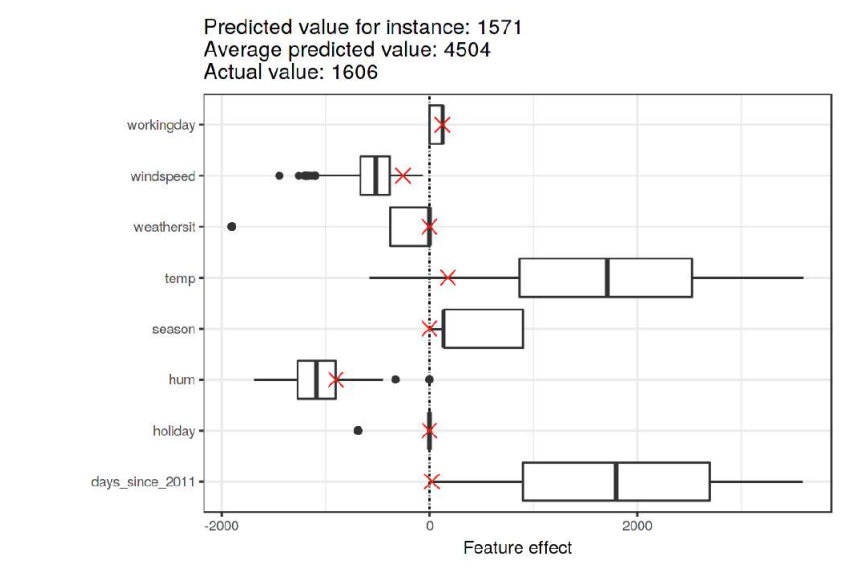
\includegraphics[width=0.7\linewidth]{Images/effect_collectif.png}
\begin{center}
    \textbf{Figure 3:} Comparaison individuel/collectif avec les boîtes à moustache 
\end{center}

\subsubsection{Codage des variables catégorielles}
Il existe plusieurs façons de coder une variable catégorielle, et le choix influence l'interprétation des poids.

Le standard dans les modèles de régression linéaire est le codage traitement, qui est suffisant dans la plupart des cas. Utiliser différents codages revient à créer différentes matrices (de conception) à partir d'une seule colonne avec la variable catégorielle. Cette section présente trois codages différents, mais il en existe bien d'autres. L'exemple utilisé comporte six instances et une variable catégorielle avec trois catégories. Pour les deux premières instances, la variable prend la catégorie A; pour les instances trois et quatre, la catégorie B; et pour les deux dernières instances, la catégorie C.

\textbf{Codage traitement}
Dans le codage traitement, le poids par catégorie est la différence estimée dans la prédiction entre la catégorie correspondante et la catégorie de référence. L'intercept du modèle linéaire est la moyenne de la catégorie de référence (lorsque toutes les autres variables restent les mêmes). La première colonne de la matrice de conception est l'intercept, qui est toujours 1. La deuxième colonne indique si l'instance i est dans la catégorie B, la troisième colonne indique si elle est dans la catégorie C. Il n'est pas nécessaire d'avoir une colonne pour la catégorie A, car alors l'équation linéaire serait sur-spécifiée et aucune solution unique pour les poids ne pourrait être trouvée. Il suffit de savoir qu'une instance n'est ni dans la catégorie B ni dans la C.
\[ 
\begin{pmatrix} 1 & 0 & 0 \\ 1 & 0 & 0 \\ 1 & 1 & 0 \\ 1 & 1 & 0 \\ 1 & 0 & 1 \\ 1 & 0 & 1 \end{pmatrix} 
\]

\textbf{Codage effet}
Le poids par catégorie est la différence y estimée de la catégorie correspondante à la moyenne générale (étant donné que toutes les autres variables sont zéro ou la catégorie de référence). La première colonne est utilisée pour estimer l'intercept. Le poids \(\beta_{0}\) associé à l'intercept représente la moyenne globale et \(\beta_{1}\), le poids pour la colonne deux, est la différence entre la moyenne générale et la catégorie B. L'effet total de la catégorie B est \(\beta_{0}+\beta_{1}\). L'interprétation pour la catégorie C est équivalente. Pour la catégorie de référence A, \(-(\beta_{1}+\beta_{2})\) est la différence avec la moyenne générale et \(\beta_{0}-(\beta_{1}+\beta_{2})\) l'effet global.
\[ 
\begin{pmatrix} 1 & -1 & -1 \\ 1 & -1 & -1 \\ 1 & 1 & 0 \\ 1 & 1 & 0 \\ 1 & 0 & 1 \\ 1 & 0 & 1 \end{pmatrix} 
\]

\textbf{Codage factice (Dummy coding)}
Le \(\beta\) par catégorie est la valeur moyenne estimée de y pour chaque catégorie (étant donné que toutes les autres valeurs des variables sont zéro ou la catégorie de référence). Notez que l'intercept a été omis ici afin qu'une solution unique puisse être trouvée pour les poids du modèle linéaire. Une autre façon de pallier ce problème de multicollinéarité est de laisser de côté l'une des catégories.
\[ 
\begin{pmatrix} 1 & 0 & 0 \\ 1 & 0 & 0 \\ 0 & 1 & 0 \\ 0 & 1 & 0 \\ 0 & 0 & 1 \\ 0 & 0 & 1 \end{pmatrix} 
\]

\subsubsection{Les modèles linéaires fournissent-ils de bonnes explications?}

Les modèles sont contrastés, mais l'instance de référence est un point de données où toutes les variables numériques sont nulles et les variables catégorielles sont à leurs catégories de référence. C'est généralement une instance artificielle et sans signification qui est peu susceptible de se produire dans vos données ou dans la réalité. Il y a une exception : si toutes les variables numériques sont centrées sur la moyenne (variable moins la moyenne de la variable) et que toutes les variables catégorielles sont codées par effet, l'instance de référence est le point de données où toutes les variables prennent la valeur moyenne de la variable. Ce pourrait aussi être un point inexistant, mais il pourrait au moins être plus probable ou plus significatif. Dans ce cas, les poids multipliés par les valeurs des variables (effets des variables) expliquent la contribution au résultat prédit contrasté avec le "point moyen". Un autre aspect d'une bonne explication est la sélectivité, qui peut être obtenue dans les modèles linéaires en utilisant moins de variables ou en formant des modèles linéaires clairsemés. Mais par défaut, les modèles linéaires ne créent pas d'explications sélectives. Les modèles linéaires créent des explications véridiques, tant que l'équation linéaire est un modèle approprié pour la relation entre les variables et le résultat.

\subsubsection{Sparse Linear Models}

Dans la réalité, il se pourrait que vous n'ayez pas seulement quelques variables, mais des centaines voire des milliers. La bonne nouvelle est qu'il existe des moyens d'introduire de la parcimonie (c'est-à-dire peu de variables) dans les modèles linéaires.
\newline
\textbf{Lasso:}
\newline

Le Lasso ajoute un terme au problème d'optimisation. La formule est la suivante :

\[
\min_{\boldsymbol{\beta}}\left(\frac{1}{n}\sum_{i=1}^n(y^{(i)}-x_{i}^T\boldsymbol{\beta})^2+\lambda||\boldsymbol{\beta}||_1\right)
\]

Ici, le terme $||\boldsymbol{\beta}||_1$, qui est la norme L1 du vecteur de variables, conduit à une pénalisation des poids importants. Avec une pénalité croissante des poids, de moins en moins de variables reçoivent une estimation de poids non nulle. Ces courbes sont également appelées chemins de régularisation. Le nombre affiché au-dessus du graphique est le nombre de poids non nuls.

\begin{center}
    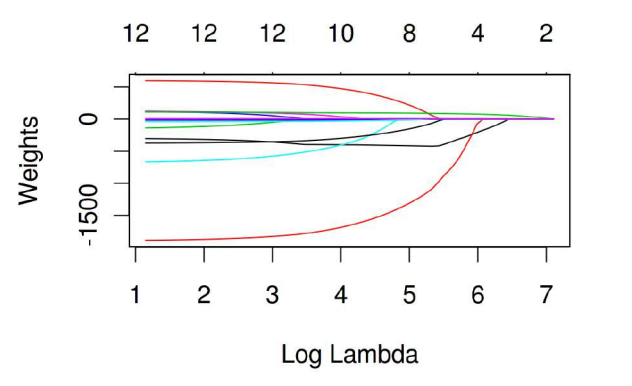
\includegraphics[width=0.7\linewidth]{Images/lasso.png} 
    \newline
    \textbf{Figure 4:} Introduction de sparsité avec le Lasso
\end{center}
Mais quelle valeur devrions-nous choisir pour $\lambda$ ? Si vous considérez le terme de pénalisation comme un paramètre de réglage (tuning parameter), alors vous pouvez trouver la valeur de $\lambda$ qui minimise l'erreur du modèle avec une cross validation.

\newline
\textbf{Lasso: Autres méthodes pour la parcimonie dans les modèles linéaires:}
\newline

\textbf{Méthodes de prétraitement}

\begin{itemize}
    \item Sélection manuelle des variables.
    \item Sélection univariée : Un exemple est le coefficient de corrélation. On ne prend en compte que les variables qui dépassent un certain seuil de corrélation entre la variable et la cible. L'inconvénient est qu'il ne considère que les variables individuellement.
\end{itemize}
\\
\textbf{Méthodes pas-à-pas (Step-wise)}
\\
\begin{itemize}
    \item Sélection avant (Forward selection) : Ajustez le modèle linéaire avec une seule variable. Faites cela avec chaque variable. Sélectionnez le modèle qui fonctionne le mieux (par exemple, le R-carré le plus élevé). Ensuite, pour les variables restantes, ajustez différentes versions de votre modèle en ajoutant chaque variable à votre meilleur modèle actuel. Sélectionnez celui qui donne les meilleurs résultats. Continuez jusqu'à ce qu'un critère soit atteint, comme le nombre maximum de variables dans le modèle.
    \item Sélection arrière (Backward selection) : Similaire à la sélection avant. Mais au lieu d'ajouter des variables, commencez par le modèle qui contient toutes les variables et essayez de déterminer quelle variable vous devez supprimer pour obtenir la plus grande augmentation de performance. Répétez cela jusqu'à ce qu'un critère d'arrêt soit atteint.
\end{itemize}

\subsubsection{Avantages et Désavantages}

\textbf{Avantages}

\begin{itemize}
    \item La modélisation des prédictions sous forme de somme pondérée rend transparente la manière dont les prédictions sont produites.
    \item Il existe un haut niveau d'expérience et d'expertise collective.
    \item Mathématiquement, il est simple d'estimer les poids et vous avez la garantie de trouver des poids optimaux.
\end{itemize}

\textbf{Désavantages}

\begin{itemize}
    \item Chaque non-linéarité ou interaction doit être créée manuellement et explicitement donnée au modèle en tant que variable d'entrée.
    \item La performance prédictive n'est pas toujours la meilleure.
    \item L'interprétation d'un poids peut être contre-intuitive car elle dépend de toutes les autres variables.
\end{itemize}

\subsection{Régression logistique}

La régression logistique modélise les probabilités pour les problèmes de classification avec deux issues possibles. C'est une extension du modèle de régression linéaire pour les problèmes de classification.

\newline
Qu'est-ce qui ne va pas avec la régression linéaire pour la classification?
\newline
Un modèle linéaire ne produit pas de probabilités. De plus, un modèle linéaire extrapole et donne des valeurs inférieures à zéro et supérieures à un. C'est un bon signe qu'il pourrait y avoir une approche plus intelligente pour la classification.

\subsubsection{Théorie}

Au lieu d'ajuster une ligne droite ou un hyperplan, le modèle de régression logistique utilise la fonction logistique pour compresser la sortie d'une équation linéaire entre 0 et 1. La fonction logistique est définie comme suit:

\[
\text{logistic}(\eta)=\frac{1}{1+\exp(-\eta)}
\]
Et elle ressemble à cela:
\begin{figure}
    \centering
    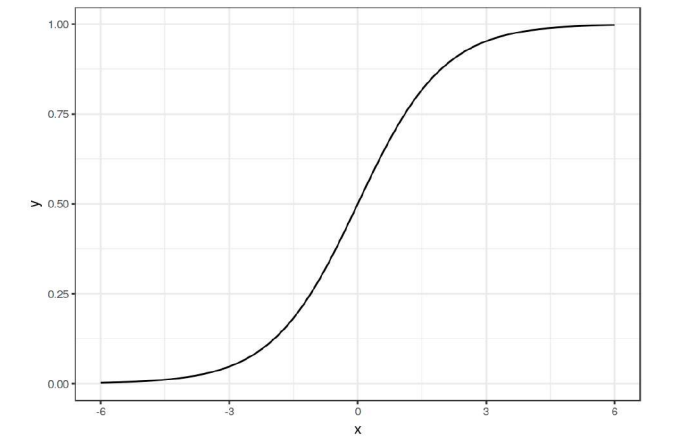
\includegraphics[width=0.5\linewidth]{Images/logisitc_function.png}
    \\
    \emph{Figure 5: Fonction logistique}
    \\
\end{figure}
\\
Ainsi, le modèle est:

\[
P(y^{(i)}=1)=\frac{1}{1+\exp(-(\beta_{0}+\beta_{1}x^{(i)}_{1}+\ldots+\beta_{p}x^{(i)}_{p}))}
\]

\subsubsection{Interprétation}

La somme pondérée est transformée par la fonction logistique en une probabilité. Par conséquent, nous devons reformuler l'équation pour l'interprétation de manière à ce que seul le terme linéaire soit du côté droit de la formule.

\[
\ln\left(\frac{P(y=1)}{1-P(y=1)}\right)=\log\left(\frac{P(y=1)}{P(y=0)}\right)=\beta_{0}+\beta_{1}x_{1}+\ldots+\beta_{p}x_{p}
\]

On appelle le terme dans la fonction \textit{ln()} les "odds" (probabilité de l'événement divisée par la probabilité de non-événement). Cela implique que:

\[
\frac{\text{odds}_{x_j+1}}{\text{odds}_{x_j}}=\exp\left(\beta_{j}(x_{j}+1)-\beta_{j}x_{j}\right)=\exp\left(\beta_j\right)
\]

Un changement dans une variable d'une unité change le rapport de odds (multiplicatif) par un facteur de \(\exp(\beta_j)\). Voici les interprétations pour le modèle de régression logistique avec différents types de variables:

\begin{itemize}
    \item Variable numérique: Si vous augmentez la valeur de la variable \(x_j\) d'une unité, les odss estimées changent par un facteur de \(\exp(\beta_j)\).
    \item Variable catégorielle binaire: L'une des deux valeurs de la variable est la catégorie de référence (dans certaines langues, celle codée en 0). Changer la variable \(x_j\) de la catégorie de référence à l'autre catégorie change les odds estimées par un facteur de \(\exp(\beta_j)\).
    \item Intercept \(\beta_0\): Lorsque toutes les variables numériques sont à zéro et que les variables catégorielles sont à la catégorie de référence, les odds estimées sont \(\exp(\beta_0)\).
\end{itemize}

\subsubsection{Avantages et Inconvénients}

De nombreux avantages et inconvénients du modèle de régression linéaire s'appliquent également au modèle de régression logistique. Son expressivité est trop restrictive (par exemple, les interactions doivent être ajoutées manuellement) et d'autres modèles peuvent avoir de meilleures performances prédictives. Un autre inconvénient du modèle de régression logistique est que l'interprétation est plus difficile car l'interprétation des poids est multiplicative et non additive.

\subsection{GLM, GAM et plus}

La plus grande force mais aussi la plus grande faiblesse du modèle de régression linéaire est que la prédiction est modélisée comme une somme pondérée des variables. De plus, le modèle linéaire est accompagné de nombreuses autres hypothèses. La mauvaise nouvelle (enfin, pas vraiment une nouvelle) est que toutes ces hypothèses ne sont presque jamais respectées dans la réalité. 

\subsubsection{Solutions aux problèmes}
\\
\textbf{Résultats non-Gaussiens – GLMs}
\\
Le concept central des modèles linéaires généralisés (ou GLMs) est de conserver la somme pondérée des variables, mais d'autoriser des distributions de résultats non gaussiens.
Le modèle est le suivant :
\[
g(E_Y(y|x))=\beta_0+\beta_1x_{1}+\ldots+\beta_px_{p}
\]

Les GLMs se composent de trois composantes: la fonction de lien \(g\), la somme pondérée \(X^T\beta\) et une distribution de probabilité de la famille exponentielle qui définit \(E_Y\).
Ainsi n'importe quelle distribution peut être modélisée pour vottre GLM. Selon la nature de la prédiction vous devez alors choisir la bonne prédiction:
\begin{itemize}
    \item Comptage de quelque chose : Distribution de Poisson
    \item Prédiction toujours positive : Distribution Exponentielle
    \item ...
\end{itemize}

\\
\textbf{Effets non linéaires - GAMs}
\\

Vous pouvez modéliser des relations non linéaires en utilisant l'une des techniques suivantes:
\begin{itemize}
    \item Transformation simple de la variable (par exemple, logarithme).
    \item Catégorisation de la variable.
    \item Modèles additifs généralisés (GAMs).
\end{itemize}

\\
Transformation de variable:
\\
Souvent, le logarithme de la variable est utilisé comme transformation. L'interprétation de la variable change en fonction de la transformation sélectionnée. Lorsque vous utilisez un GLM avec une fonction de lien qui n'est pas la fonction d'identité, alors l'interprétation devient plus compliquée, car vous devez incorporer les deux transformations dans l'interprétation (sauf si elles s'annulent mutuellement, comme le log et exp, alors l'interprétation devient plus facile).

\\
Catégorisation de variable
\\
Une autre possibilité pour obtenir un effet non linéaire est de discrétiser la variable. Le problème avec cette approche est qu'elle nécessite plus de données, elle est plus susceptible de faire de l'overfit et il n'est pas clair comment discrétiser la variable de manière significative (intervalles équidistants ou quantiles ? combien d'intervalles ?).

\\
Modèles additifs généralisés (GAMs)
\\
Les GAMs relâchent la restriction selon laquelle la relation doit être une simple somme pondérée, et supposent au lieu de cela que le résultat peut être modélisé par une somme de fonctions arbitraires de chaque variable.
\[ g(E_Y(y|x)) = \beta_0 + f_1(x_1) + f_2(x_2) + \ldots + f_p(x_p) \]
La grande question est de savoir comment apprendre des fonctions non linéaires. La réponse s'appelle ``splines'' ou ``fonctions spline''. Les splines sont des fonctions qui sont construites à partir de fonctions de base plus simples.

\subsubsection{Avantages}
Quels que soient les problèmes que vous rencontrez avec les modèles linéaires, vous trouverez probablement une extension qui le résout.

\subsubsection{Inconvénients}
Le nombre impressionnant de façons dont vous pouvez étendre le simple modèle linéaire est accablant, et pas seulement pour les débutants. La plupart des modifications du modèle linéaire rendent le modèle moins interprétable. Les GLMs, GAMs, et autres reposent sur des hypothèses concernant le processus générant les données. Si celles-ci ne sont pas respectées, l'interprétation des poids n'est plus valide.

\subsubsection{Autres extensions}
\begin{itemize}
    \item Violation de l'hypothèse d'indépendance : Rechercher les modèles mixtes ou les équations d'estimation généralisées.
    \item Hétéroscédasticité ou présence d'Outliers: Rechercher la régression robuste.
    \item Prédiction du temps avant un événement: Rechercher les modèles de survie paramétriques, la régression de Cox.
    \item Résultat à prédire est une catégorie: régression multinomiale.
    \item Prédiction de catégories ordonnées: Rechercher le modèle "of proportional odds".
    \item La vériable prédite est un compte: Régression de Poisson.
    \item Données manquantes: imputation multiple.
    \item Intégration de connaissances antérieures: inférence bayésienne.
\end{itemize}



\subsection{Arbre de décision}

L'algorithme de classification et d'arbres de régression (CART ou Classification and Regression Trees) est probablement l'algorithme le plus populaire pour l'induction d'arbres. Nous nous concentrerons sur CART, mais l'interprétation est similaire pour la plupart des autres types d'arbres.

\begin{center}
    \centering
    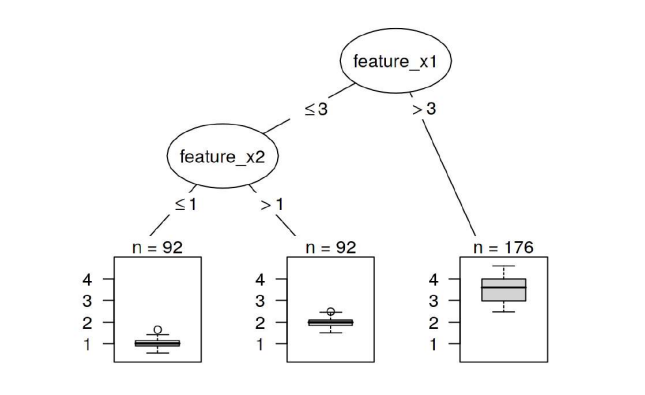
\includegraphics[width=0.5\linewidth]{Images/cart.png}
    \\
    \emph{Figure 6: Abre de Classification}
    \\
\end{center}
\\
La formule suivante décrit la relation entre le résultat \(y\) et les variables \(x\).
\[ \hat{y} = \hat{f}(x) = \sum_{m=1}^M c_m I\{x \in R_m\} \]
Chaque instance tombe exactement dans un nœud feuille (= sous-ensemble \(R_m\)).
\[ I\{x \in R_m\} \] est la fonction identité qui renvoie 1 si \(x\) est dans le sous-ensemble \(R_m\) et 0 sinon.
\\
Si une instance tombe dans un nœud feuille \(R_l\), le résultat prédit est \(\hat{y} = c_l\), où \(c_l\) est la moyenne de toutes les instances d'entraînement dans le nœud feuille \(R_l\).
Mais d'où viennent ces sous-ensembles ? C'est assez simple : CART prend une variable et détermine quel point de coupure minimise la variance de \(y\) pour une tâche de régression ou l'indice de Gini de la distribution des classes de \(y\) pour les tâches de classification. La variance et l'indice de Gini sont minimisés lorsque les points de données dans les nœuds ont des valeurs très similaires pour \(y\).

\subsubsection{Interprétation}
En partant du nœud racine, vous allez aux nœuds suivants et les arêtes vous indiquent quels sous-ensembles vous examinez. Une fois que vous atteignez le nœud feuille, le nœud vous indique le résultat prédit. Toutes les arêtes sont connectées par ``AND''.

\subsubsection{Importance de la variable}
L'importance globale d'une variable dans un arbre de décision peut être calculée de la manière suivante : parcourez tous les splits pour lesquels la variable a été utilisée et mesurez combien elle a réduit la variance ou l'indice de Gini par rapport au nœud parent. La somme de toutes les importances est mise à l'échelle à 100.

\paragraph{Décomposition de l'arbre}
\[ \hat{f}(x) = \bar{y} + \sum_{d=1}^D \text{split.contrib}(d,x) = \bar{y} + \sum_{j=1}^p \text{feat.contrib}(j,x) \]
La prédiction d'une instance individuelle est la moyenne de la valeur cible plus la somme de toutes les contributions des \(D\) splits qui se produisent entre le nœud racine et le nœud terminal où l'instance se termine. Nous ne sommes pas intéressés par les contributions des splits, mais par les contributions des variables. Une variable peut être utilisée pour plusieurs splits ou pas du tout. Nous pouvons ajouter les contributions pour chacune des \(p\) variables et obtenir une interprétation de la contribution de chaque variable à une prédiction.

\subsubsection{Avantages}
\begin{itemize}
    \item La structure de l'arbre est idéale pour capter les interactions entre les variables dans les données.
    \item On interprète \(n\) groupes distincts qui sont souvent plus faciles à comprendre que des points sur un hyperplan multidimensionnel comme dans la régression linéaire.
    \item La structure de l'arbre a également une visualisation naturelle, avec ses nœuds et ses arêtes.
    \item Les arbres créent de bonnes explications
    \item Les arbres invitent à réfléchir aux valeurs prédites pour des instances individuelles comme des contre-factuels.
    \item Il n'est pas nécessaire de transformer les variables.
\end{itemize}

\subsubsection{Inconvénients}
\begin{itemize}
    \item Les arbres ne parviennent pas à traiter les relations linéaires.
    \item De légères modifications dans la variable d'entrée peuvent avoir un grand impact sur le résultat prédit.
    \item Les arbres de décision sont très interprétables tant qu'ils sont courts. Le nombre de nœuds terminaux augmente rapidement avec la profondeur.
\end{itemize}

\subsection{Règles de décision}

Une règle de décision est une simple déclaration IF-THEN composée d'une condition et d'une prédiction. L'utilité d'une règle de décision est généralement résumée en deux nombres : le support et la précision.

\paragraph{Support ou couverture d'une règle}
Le pourcentage d'instances auxquelles s'applique la condition d'une règle est appelé le support. Prenons par exemple la règle taille=grand ET emplacement=bon ALORS valeur=élevée pour prédire les valeurs des maisons. Supposons que 100 des 1000 maisons sont grandes et bien situées, alors le support de la règle est de 10\%.

\paragraph{Précision ou confiance d'une règle}
La précision d'une règle est une mesure de la justesse de la règle pour prédire la bonne classe pour les instances auxquelles s'applique la condition de la règle. Par exemple : supposons que sur les 100 maisons, où la règle taille=grand ET emplacement=bon ALORS valeur=élevée s'applique, 85 ont une valeur=élevée, 14 ont une valeur=moyenne et 1 a une valeur=faible, alors la précision de la règle est de 85\%. En ajoutant plus de caractéristiques à la condition, nous pouvons obtenir une meilleure précision, mais perdons en support.

\paragraph{Problèmes potentiels}
Lors de la création d'un classificateur, vous pouvez rencontrer l'un des problèmes suivants :
\begin{itemize}
    \item Les règles peuvent se chevaucher.
    \item Aucune règle ne s'applique.
\end{itemize}
Il existe deux principales stratégies pour combiner plusieurs règles : les listes de décision (ordonnées) et les ensembles de décision (non ordonnés, pouvoir de vote pour chaque règle puis vote majoritaire).

\paragraph{Apprendre des règles à partir de données}
Il existe de nombreuses façons d'apprendre des règles à partir de données et ce papier est loin de toutes les couvrir. Nous nous pencherons sur les deux première méthodes des trois suivantes :
\begin{enumerate}
    \item OneR apprend des règles à partir d'une seule caractéristique. OneR se caractérise par sa simplicité, son interprétabilité et son utilisation comme référence.
    \item La couverture séquentielle est une procédure générale qui apprend itérativement des règles et supprime les points de données couverts par la nouvelle règle. Cette procédure est utilisée par de nombreux algorithmes d'apprentissage de règles.
    \item Les listes de règles bayésiennes combinent des motifs fréquemment pré-établis dans une liste de décision en utilisant la statistique bayésienne. L'utilisation de motifs pré-établis est une approche courante utilisée par de nombreux algorithmes d'apprentissage de règles. 
\end{enumerate}



\subsubsection{Apprendre des règles à partir d'une seule caractéristique (OneR)}

L'algorithme est simple et rapide:
\begin{enumerate}
    \item Discrétiser les caractéristiques continues en choisissant des intervalles appropriés.
    \item Pour chaque caractéristique:
    \begin{itemize}
        \item Créer un tableau croisé entre les valeurs de la caractéristique et le résultat (catégoriel).
        \item Pour chaque valeur de la caractéristique, créer une règle qui prédit la classe la plus fréquente des instances ayant cette valeur de caractéristique particulière (peut être lue à partir du tableau croisé).
        \item Calculer l'erreur totale des règles pour la caractéristique.
    \end{itemize}
    \item Sélectionner la caractéristique avec la plus petite erreur totale.
\end{enumerate}
OneR préfère les caractéristiques avec de nombreux niveaux possibles, car ces caractéristiques peuvent surajuster la cible plus facilement. Une solution serait de diviser les données en ensembles d'entraînement et de validation, d'apprendre les règles sur les données d'entraînement et d'évaluer l'erreur totale pour choisir la caractéristique sur l'ensemble de validation.

\subsubsection{Couverture séquentielle}

La couverture séquentielle est une procédure générale qui apprend une seule règle à plusieurs reprises pour créer une liste de décision (ou ensemble) qui couvre l'ensemble des données règle par règle. Supposons que nous ayons déjà un algorithme capable de créer une seule règle couvrant une partie des données. L'algorithme est le suivant:
\begin{itemize}
    \item Commencer avec une liste vide de règles (rliste).
    \item Apprendre une règle r.
    \item Tant que la liste des règles est en dessous d'un certain seuil de qualité (ou que les exemples positifs ne sont pas encore couverts):
    \begin{itemize}
        \item Ajouter la règle r à rliste.
        \item Supprimer tous les points de données couverts par la règle r.
        \item Apprendre une autre règle sur les données restantes.
    \end{itemize}
    \item Renvoyer la liste de décision.
\end{itemize}


\begin{center}
    \centering
    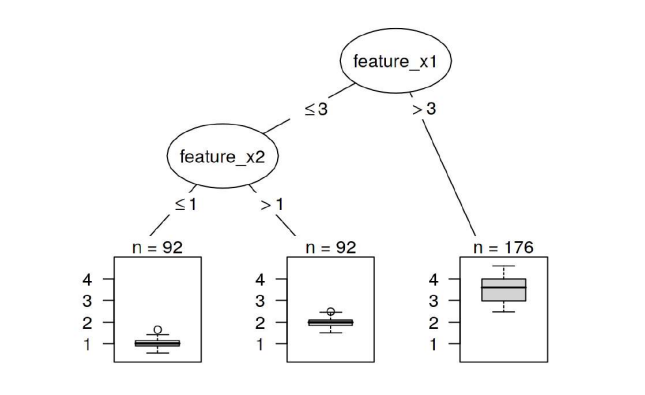
\includegraphics[width=0.5\linewidth]{Images/cart.png}
    \\
    \emph{Figure 7: Couverture séquentielle}
    \\
\end{center}
\\
\paragraph{Comment apprend-on une seule règle?}
 L'algorithme OneR serait inutile ici, car il couvrirait toujours tout l'espace des caractéristiques. Mais il existe de nombreuses autres possibilités. Une possibilité est d'apprendre une seule règle à partir d'un arbre de décision avec une recherche en faisceau:
\begin{itemize}
    \item Apprendre un arbre de décision (avec CART ou un autre algorithme d'apprentissage d'arbre).
    \item Commencer à la racine et sélectionner récursivement le nœud le plus pur (par exemple, avec le taux de mauvaise classification le plus faible).
    \item La classe majoritaire du nœud terminal est utilisée comme prédiction de la règle; le chemin menant à ce nœud est utilisé comme condition de la règle.
\end{itemize}
La figure suivante illustre la recherche en faisceau dans un arbre:

\begin{center}
    \centering
    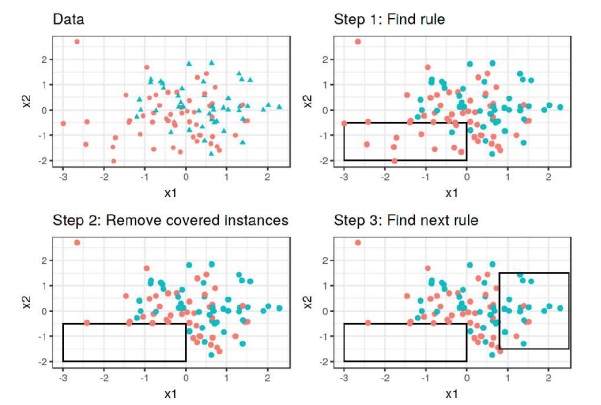
\includegraphics[width=0.7\linewidth]{Images/rule_elimantion.png}
    \\
    \emph{Figure 8: Couverture séquentielle}
    \\
\end{center}
\\
RIPPER (Repeated Incremental Pruning to Produce Error Reduction) par Cohen (1995) est une variante de l'algorithme de couverture séquentielle. RIPPER est un peu plus sophistiqué et utilise une phase de post-traitement (élagage des règles) pour optimiser la liste (ou l'ensemble) de décision. RIPPER peut fonctionner en mode ordonné ou non ordonné et générer soit une liste de décision, soit un ensemble de décision.


\subsubsection{Avantages}
Voici quelques-uns des avantages des règles IF-THEN en général :
\begin{itemize}
    \item Facilité d'interprétation : Cette affirmation est vraie uniquement si le nombre de règles est faible, que les conditions des règles sont courtes (maximum 3, dirais-je) et que les règles sont organisées dans une liste de décision ou un ensemble de décision non superposé.
    \item Aussi expressives que les arbres de décision, tout en étant plus compactes.
    \item La prédiction avec des règles IF-THEN est rapide.
    \item Robustes face aux transformations monotones.
    \item Génèrent généralement des "sparse models", ce qui signifie que peu de caractéristiques sont incluses. Ils ne sélectionnent que les caractéristiques pertinentes pour le modèle.
\end{itemize}

\subsubsection{Inconvénients}
Les règles de décision ne sont pas sans inconvénients :
\begin{itemize}
    \item Elles se concentrent sur la classification et négligent presque complètement la régression.
    \item Souvent, les caractéristiques doivent également être catégorielles.
    \item Les règles de décision sont mauvaises pour décrire les relations linéaires.
\end{itemize}

\subsection{Autres Modèles Interprétables}

\subsubsection{Classificateur Naive Bayes}
Le classificateur Naive Bayes calcule les probabilités de classe pour chaque caractéristique indépendamment, ce qui équivant à une hypothèse de forte indépendance des caractéristiques.
\begin{equation}
P(C_k|x) = \frac{1}{Z} P(C_k) \prod_{i=1}^n P(x_i|C_k)
\end{equation}
Naive Bayes est un modèle interprétable en raison de l'hypothèse d'indépendance.
Il peut être interprété au niveau modulaire.

\subsubsection{K-Plus Proches Voisins (K-Nearest Neighbors)}
La méthode des k-plus proches voisins peut être utilisée pour la régression et la classification et utilise les voisins les plus proches d'un point de données pour la prédiction. Pour la classification, la méthode des k-plus proches voisins attribue la classe la plus commune des voisins les plus proches d'une instance.
\begin{itemize}
    \item Algorithme d'apprentissage basé sur les instances, le modèle est intrinsèquement local.
    \item Il n'y a pas de paramètres à apprendre, donc il n'y a pas d'interprétabilité au niveau modulaire.
    \item Si une instance est constituée de centaines ou de milliers de caractéristiques, alors elle n'est pas interprétable, dirais-je. Mais si vous avez peu de caractéristiques ou un moyen de réduire votre instance aux caractéristiques les plus importantes, présenter les k-plus proches voisins peut vous donner de bonnes explications.
\end{itemize}
